As explained in the introduction,
a trade policy that led to a dispute (formally called as \textit{Government Measure}) is pretty much complicated.
For example, the Panel for the \textit{US - Offset (Byrd Amendment)} explains:

\begin{quote}
    ``The CDSOA is a new and \textbf{complex measure}, applied in a complex legal environment. In
    concluding that the CDSOA is in violation of the above mentioned provisions, we have been
    confronted by sensitive issues regarding the use of subsidies as trade remedies.
    this matter through negotiation. \ldots''
\end{quote}

\noindent To address this complexity, member who raises the claim (formally called as \textit{complainant}) usually cites multiple articles of the WTO agreements. For example, in the
\textit{US - Offset (Byrd Amendment)},
a group of complainants\footnote{Australia,
    Brazil,
    Chile,
    European Communities,
    India,
    Indonesia,
    Japan,
    Korea and Thailand}
cited articles as shown in Table \ref{xltabular:cited-article-for-us-offset} from the WTO agreements to claim possible inconsitency of CDSOA to these articles\footnote{It is worth noting that the WTO agreements comprises many different agreements covering each specific topic in trade such as \textit{Agreement on Anti-dumping, Agreement on Subsidies and Countervailing Measures} and so on.}:\\
\begin{xltabular}{\linewidth}{ l | X }
    % \caption{explain something if needed}
    % \\
    \hline

    \textbf{\normalsize Name of WTO Agreement} & \textbf{\normalsize Cited Articles}\\
    \endfirsthead
    \hline \hline

    Agreement on Anti-dumping& 1, 5.4, 8, 18.1, 18.4 \\ \hline
    General Agreement on Tariffs and Trade 1994& VI:3, X:3, XXIII:1, VI:2  \\ \hline
    Agreement on Subsidies and Countervailing Measures& 4.10, 7.9, 10, 11.4, 18, 32.1, 32.5 \\ \hline
    Agreement Establishing the World Trade Organization & XVI:4 \\ \hline
    \caption{Cited Aticles in \textit{US - Offset (Byrd Amendment)}}
    \label{xltabular:cited-article-for-us-offset}
\end{xltabular}


\noindent Upon this understanding, 
I collected two different types of data for 143 different dispute cases requested to WTO DSB.\footnote{List of collected cases is
    available at \hyperref[sub:cited-articles-table]{Appendix A.2}
}.
One is textual description of trade policy
that led to the dispute \hyperref[sub:factual-aspect-example]{(\textit{See} example at Appendix A.2)} and the other one is
set of articles of the WTO agreements that are
cited for each dispute \hyperref[sub:cited-articles-table]{(Appendix A.3)}.
I will explain the format and the content of
data with an example at the following subsections.
% Technical details about the automated way 
% of collecting data will be
% explained in the \hyperref[appendix:panel-report-toc]{Appendix A.4}.

\begin{figure}[h]
    \centering
    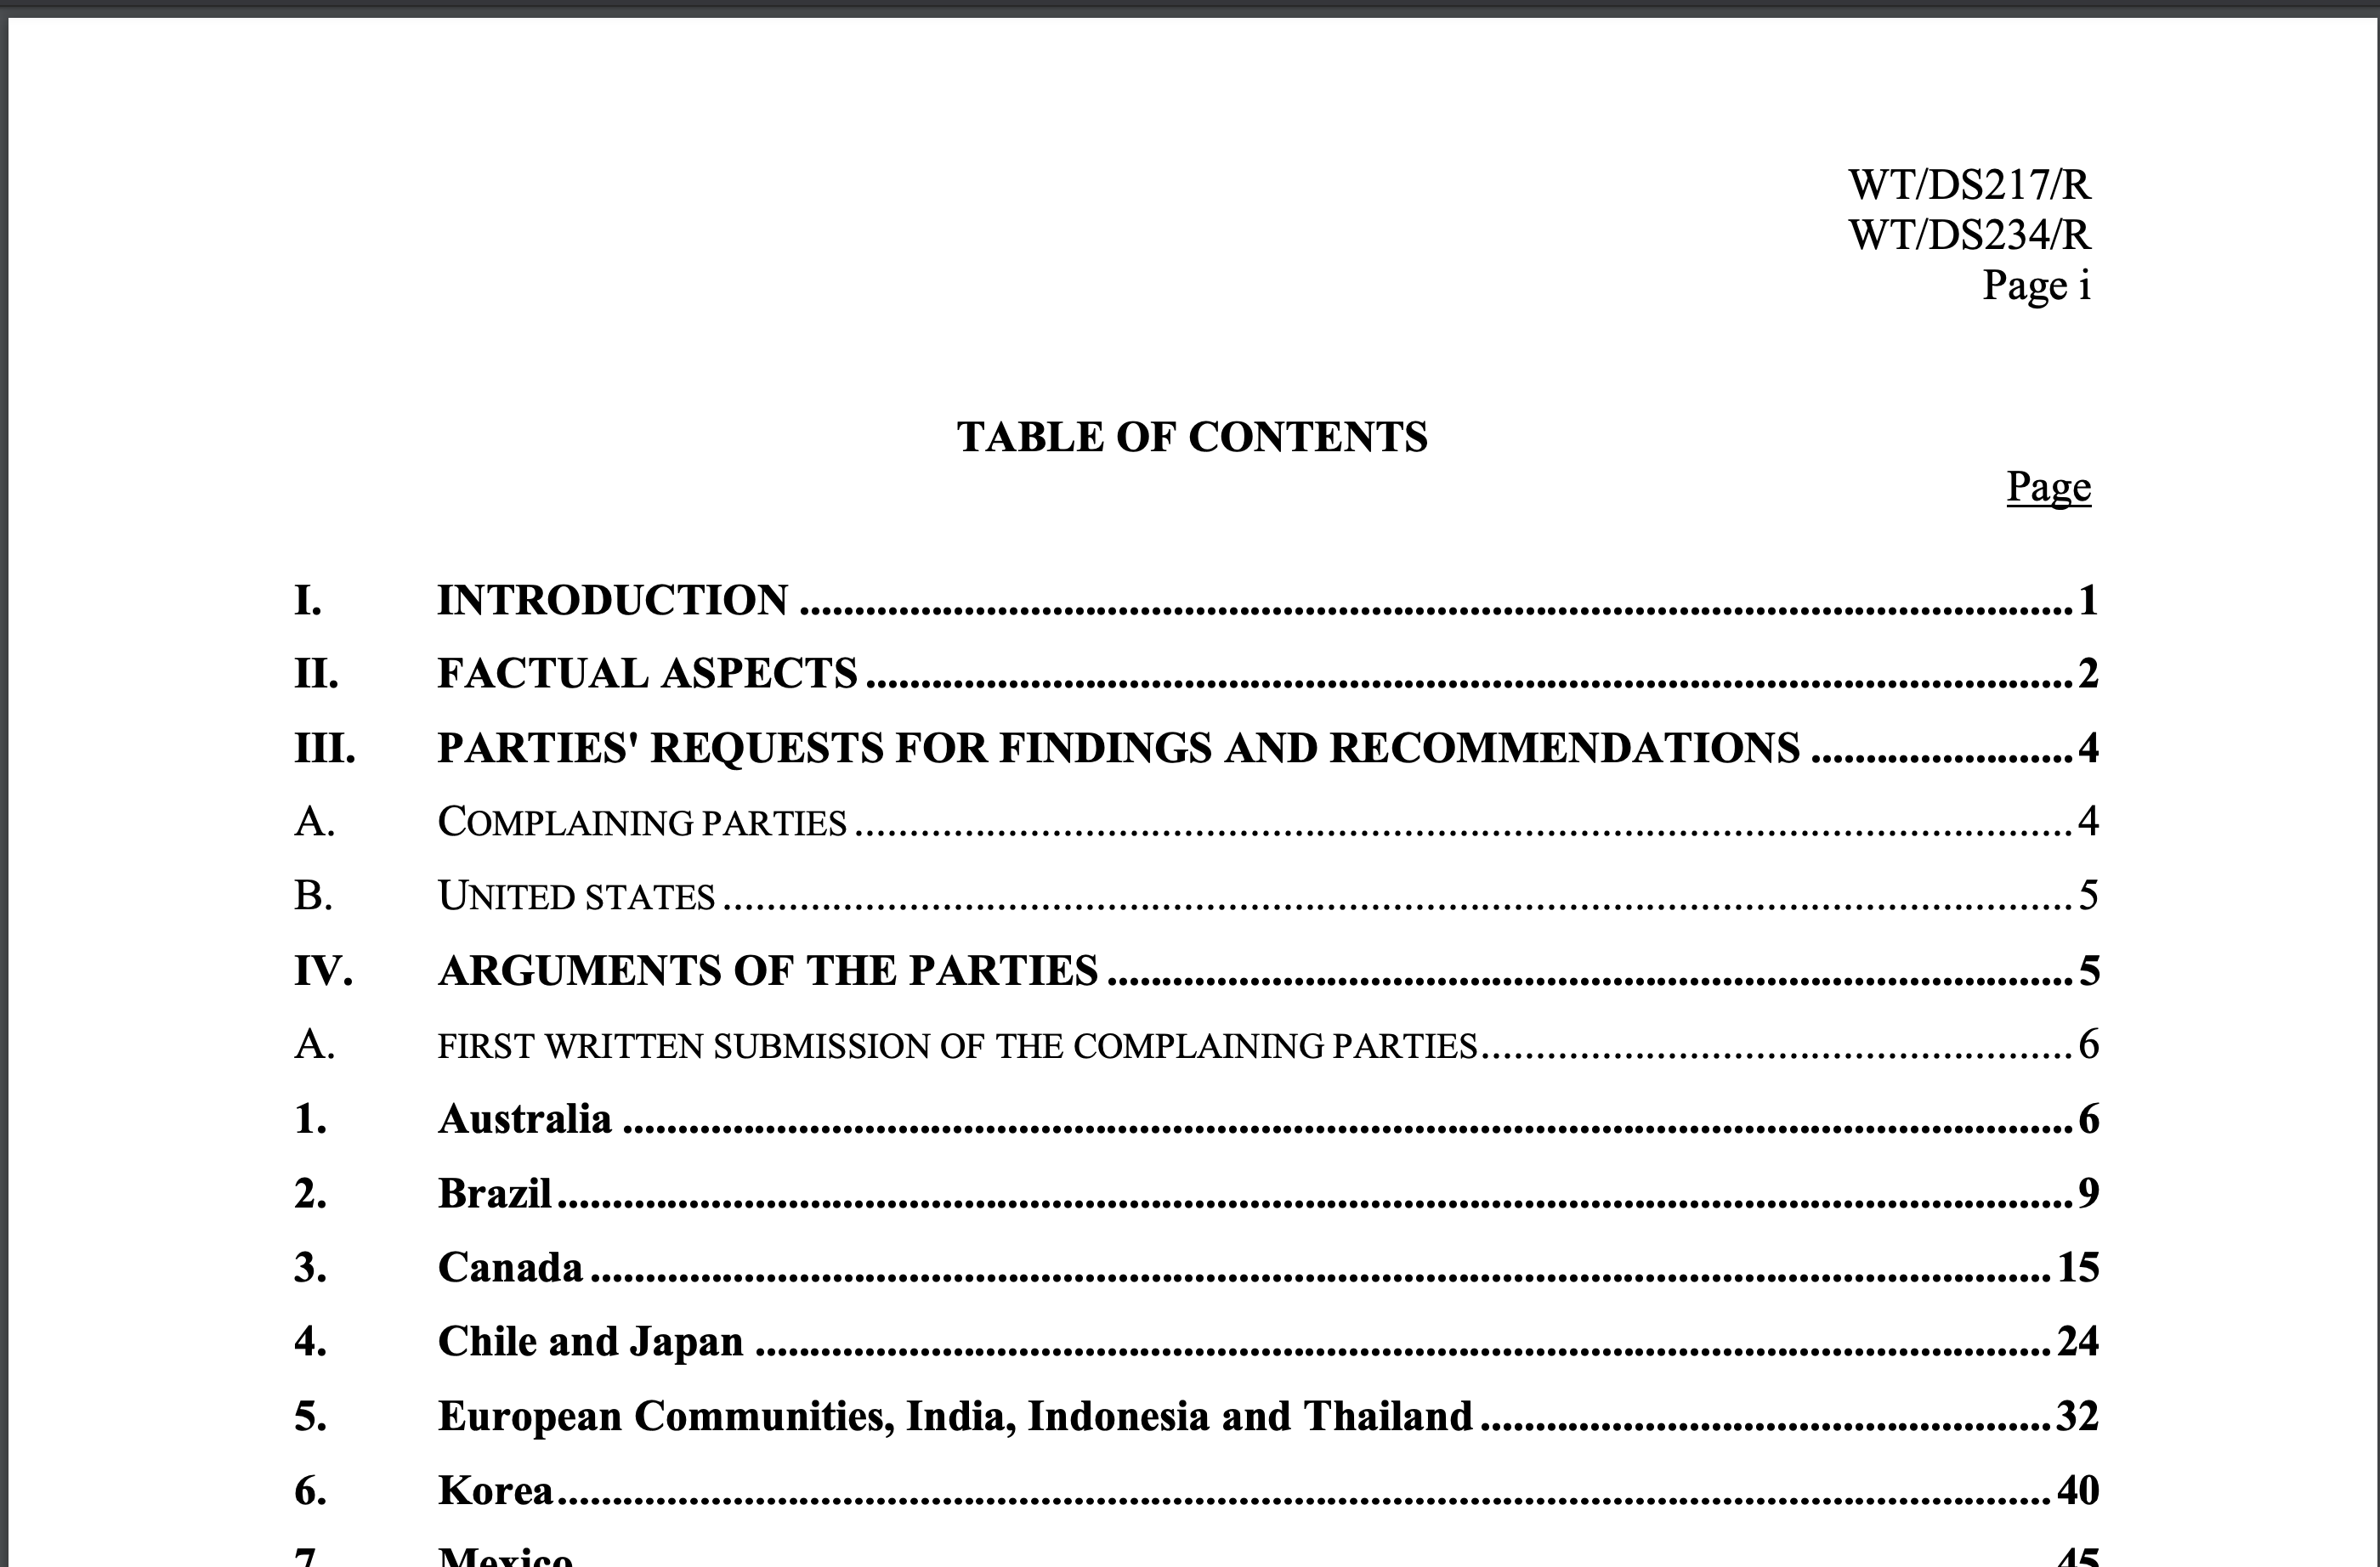
\includegraphics[scale=0.28]{Data/pngs/panel_report_toc.png}
    \caption{
        {\bf Table of Contents of Panel Report: }Panel provides 
        factual aspect in the panel report with its page location.
        }
    \label{fig:panel-report-toc}
\end{figure}
% \begin{center}
%     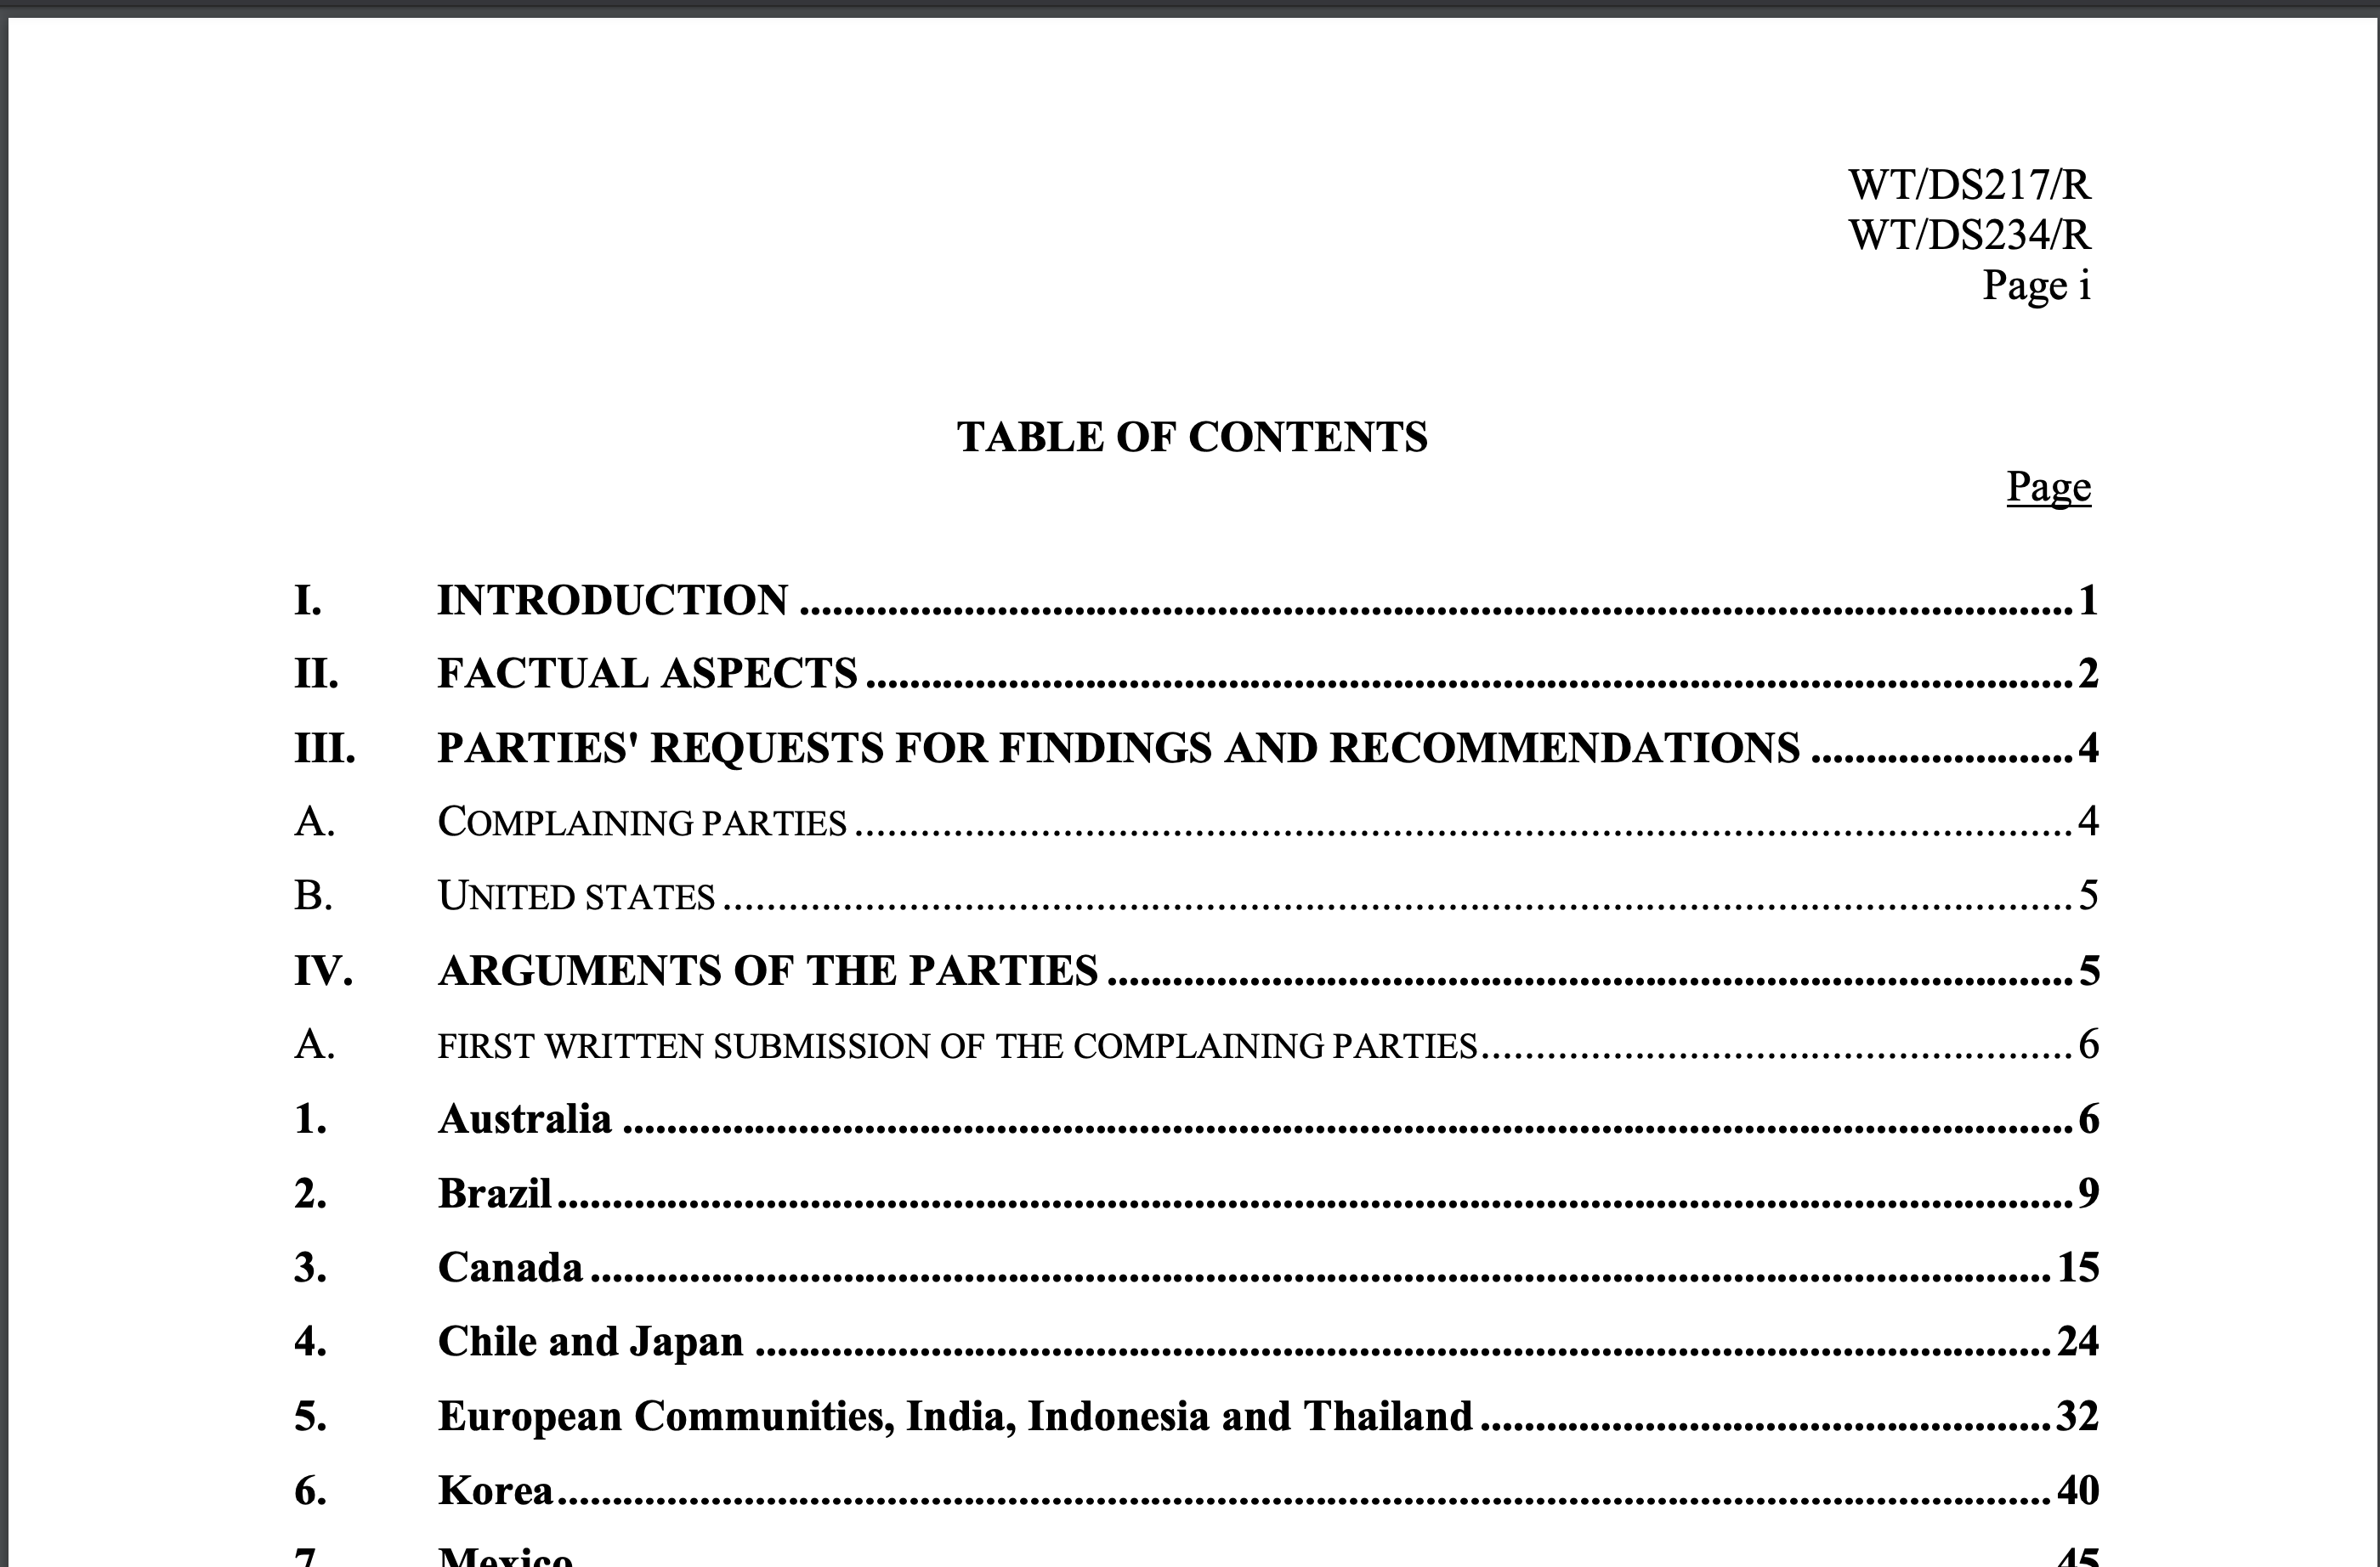
\includegraphics[scale=0.3]{Data/pngs/panel_report_toc.png}
% \end{center}


% This section explains how I collected 
% which data to train the neural network. 
% Basically, 





% I collected two different 
% types of data, one is textual description of trade policy 
% that led to the dispute and the other one is 
% set of articles of the WTO agreement that are
% cited for the dispute.s



% \begin{displayquote}
%     ``Korea' s domestic support for beef in 1997 and 1998 exceeded the de minimis level contrary to Article 6 of the Agreement on Agriculture.''
%   \end{displayquote}

%   \begin{itemize}
%     \item exemplify as detail as possible to inform readers about how data looks like.
%     \item Privide a running example that shows how WTO works with data. 
%     \item (Borrow from the previous paper)

%   \end{itemize}
